\documentclass[10pt]{article}
\usepackage[framemethod=TikZ]{mdframed}
\usepackage{amsthm}
\usepackage[landscape]{geometry}
\usepackage{multicol}
\usepackage{tikz}
\usepackage{pgfplots}
\usepackage{xcolor}
\usepackage{amsmath}
\usepackage[T1]{fontenc}
\usepackage{utopia}
\usepackage{changepage}
\usepackage{amssymb}
\usepackage{fancyhdr}
\usepackage[many]{tcolorbox}
\usepackage{moresize}
\usepackage{fullpage}
\usepackage{mathpazo}
\usepackage{tikz-3dplot}
\usepackage{cancel}
\tdplotsetmaincoords{70}{165}
\pgfplotsset{compat=1.18}

\usetikzlibrary{
    shadings, calc, patterns, angles, quotes, arrows.meta, 
    decorations.pathmorphing, decorations.pathreplacing, 
    fadings, 3d, perspective, backgrounds, intersections, 
    decorations.markings, bending
}

\usepgfplotslibrary{
    groupplots, external, colormaps, patchplots, fillbetween
}


\setlength{\baselineskip}{1.2em}
\setlength{\parskip}{-0.75em}

\makeatletter
\tikzoption{canvas is xy plane at z}[]{%
    \def\tikz@plane@origin{\pgfpointxyz{0}{0}{#1}}%
    \def\tikz@plane@x{\pgfpointxyz{1}{0}{#1}}%
    \def\tikz@plane@y{\pgfpointxyz{0}{1}{#1}}%
    \tikz@canvas@is@plane}
\makeatother

% Reds (r)
\definecolor{r1}{RGB}{255, 191, 191}    % Light coral
\definecolor{r2}{RGB}{255, 191, 223}    % Light pink
\definecolor{r3}{RGB}{255, 207, 207}    % Light rose

% Blues (b)
\definecolor{b1}{RGB}{191, 223, 255}    % Light blue
\definecolor{b2}{RGB}{191, 239, 255}    % Light sky
\definecolor{b3}{RGB}{191, 255, 255}    % Light cyan

% Greens (g)
\definecolor{g1}{RGB}{191, 255, 191}    % Light green
\definecolor{g2}{RGB}{191, 255, 223}    % Light mint
\definecolor{g3}{RGB}{207, 255, 207}    % Light sage

% Oranges (o)
\definecolor{o1}{RGB}{255, 223, 191}    % Light peach
\definecolor{o2}{RGB}{255, 239, 191}    % Light cream
\definecolor{o3}{RGB}{255, 231, 191}    % Light buff

% Violets (v)
\definecolor{v1}{RGB}{223, 191, 255}    % Light purple
\definecolor{v2}{RGB}{239, 191, 255}    % Light lilac
\definecolor{v3}{RGB}{231, 191, 255}    % Light lavender

% Yellows (y)
\definecolor{y1}{RGB}{255, 255, 191}    % Light yellow
\definecolor{y2}{RGB}{255, 247, 191}    % Light cream yellow
\definecolor{y3}{RGB}{255, 239, 191}    % Light warm cream

\definecolor{w}{HTML}{eeeeee}
\definecolor{g}{HTML}{444444}
\definecolor{b}{HTML}{222222}
\definecolor{lightgrey}{HTML}{cccccc}

\geometry{
    letterpaper,
    left=0.25in,
    right=0.25in,
    top=0.15in,
    bottom=0.25in
}


\newcommand{\hr}{\centerline{\rule{3.5in}{1pt}}}


\newcommand{\nc}[2][b]{%
\tikz \draw [draw=#1,thick]
    ($(current page.center)-(0.495\linewidth,0)$) -- 
    ($(current page.center)+(0.495\linewidth,0)$)
    node [midway, fill=b] {\ssmall\textbf{\uppercase{#2}}};
}

\newtcolorbox{conceptbox}[2][]{
	breakable,
	vfill before first=false,
	segmentation at break=false,
	size=fbox,
	colback=b,
	title=\scriptsize\textbf{\MakeUppercase{#2}},
	left=2pt,
	right=2pt,
	top=3pt,
	bottom=1pt,
	boxrule=1pt,
	coltitle=b,
	colupper=w,
	pad at break=5pt,
	toprule at break=4pt,
	bottomrule at break=0.75pt,
	colframe=#1,
	enlargepage=12in, 
	before upper*={\setlength{\baselineskip}{0.75em}\setlength{\parskip}{0em}}
}

\title{POLYMERS}
\parindent0pt

\begin{document}
\ssmall
\pagecolor{b}
\fontfamily{put}
\begin{minipage}{\textwidth}
	\tikz{
		\draw[thick, color=w] (1,0) -- (\textwidth-0.25in,0);
		\node[anchor=west, fill = b, inner sep = 3pt, text=w] at (0,0) {\textbf{POLYMERS 2}};
		\node[anchor=east, fill = b, inner sep = 3pt, text=w] at (\textwidth,0) {\textbf{CB}};
	}
\end{minipage}

\begin{multicols*}{4}
\begin{conceptbox}[v3]{Header}
	\ssmall
	\nc[v3]{Behavior}\\
	\textbf{Stress (}\(\sigma\)\textbf{):} \(\sigma = \frac{F}{A_0}\)\\[0.3em]
	\textbf{Strain (}\(\varepsilon\)\textbf{):} \(\varepsilon = \frac{\Delta L}{L_0}\)\\[0.3em]
	\textbf{Young’s Modulus (}\(E\)\textbf{):} \(E = \frac{\sigma}{\varepsilon}\) (in elastic region)\\[0.4em]
	\textbf{Shear Modulus (}\(G\)\textbf{):} \(G = \frac{\tau}{\gamma}\)\\[0.3em]
	\textbf{Poisson’s Ratio (}\(\nu\)\textbf{):} \(\nu = -\frac{\varepsilon_{\perp}}{\varepsilon_{\parallel}}\)\\[0.3em]
	\textbf{True Stress (}\(\sigma_\text{true}\)\textbf{):} \(\sigma_{\text{true}} = \frac{F}{A_{\text{instantaneous}}}\)\\[0.3em]
	\textbf{True Strain (}\(\varepsilon_\text{true}\)\textbf{):} \(\varepsilon_{\text{true}} = \ln\frac{L}{L_0}\)\\[0.3em]
	\textbf{Stress Relaxation:} \(\sigma(t) = \sigma_0 e^{-\frac{t}{\tau}}\)\\

	\tiny
	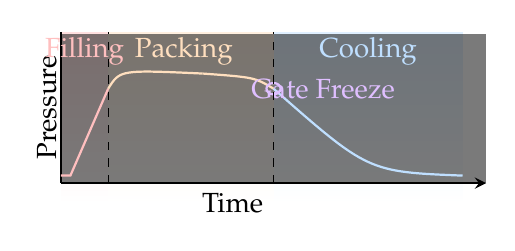
\begin{tikzpicture}[scale=0.6, yscale=0.8]
		\fill[color=r1, draw opacity=0.5, fill opacity=0.5, path fading=south] (0,-0.5) rectangle (1,4);
		\fill[o1, draw opacity=0.5, fill opacity=0.5, path fading=south] (1,-0.5) rectangle (4.5,4);
		\fill[b1, draw opacity=0.5, fill opacity=0.5, path fading=south] (4.5,-0.5) rectangle (8.5,4);
		\fill[color=b, fill opacity=0.6] (0,0) rectangle (9,3.95);
		% pvT behavior with processing stages
		\draw[-stealth, thick] (0,0) -- (9,0) node[below left, midway]{Time};
		\draw[-, thick] (0,0) -- (0,4) node[rotate=90, anchor=center] at (-0.3,2) {Pressure};

		% Processing stages
		\draw[r1,thick] (0,0.2) -- (0.2,0.2) -- (1,2.5);
		\draw[o1,thick] (1,2.5) .. controls (1.25,3) .. (3,2.9);
		\draw[o1,thick] (3,2.9) .. controls (4.1,2.8) .. (4.5,2.5);
		\draw[b1,thick] (4.5,2.5) .. controls (6.5,0.3) .. (8.5,0.2);

		\node[r1] at (0.5,3.5) {Filling};
		\node[o1] at (2.6,3.5) {Packing};
		\node[b1] at (6.5,3.5) {Cooling};

		% Gate freeze-off point
		\draw[v1,thick] (4.5,2.5) circle (0.15);
		\node[v1] at (5.55,2.5) {Gate Freeze};

		% Vertical dashed lines
		\draw[dashed] (1,0) -- (1,4);
		\draw[dashed] (4.5,0) -- (4.5,4);
	\end{tikzpicture}\\[1em]
	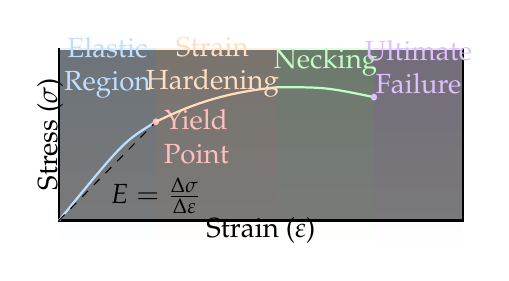
\begin{tikzpicture}[scale=0.57, yscale=1.1]
		\fill[color=b1, draw opacity=0.5, fill opacity=0.5, path fading=south] (0,-0.5) rectangle (2.16,3.5);
		\fill[o1, draw opacity=0.5, fill opacity=0.5, path fading=south] (2.16,-0.5) rectangle (4.86,3.5);
		\fill[g1, draw opacity=0.5, fill opacity=0.5, path fading=south] (4.86,-0.5) rectangle (7.02,3.5);
		\fill[v1, draw opacity=0.5, fill opacity=0.5, path fading=south] (7.02,-0.5) rectangle (9,3.5);
		\fill[color=b, fill opacity=0.6] (0,0) rectangle (9,3.45);
		% Basic stress-strain curve
		\draw[-,thick] (0,3.5) -- (0,0) -- (9,0) -- (9,3.5);
		\node at (4.5,-0.2) {Strain ($\varepsilon$)};
		\node[rotate=90] at (-0.2,1.75) {Stress ($\sigma$)};

		% Elastic region
		\draw[b1,thick] (0,0) .. controls (1.44,1.6) .. (2.16,2);
		\node[b1, align=center] at (1.08,3.1) {Elastic\\Region};
		\draw[dashed] (0,0) -- (2.16,2);
		\node at (2.16,0.5) {$E = \frac{\Delta\sigma}{\Delta\varepsilon}$};

		% Yield point
		\fill[r1] (2.16,2) circle (2pt);
		\node[r1, align=center] at (3.06,1.7) {Yield \\Point};

		% Plastic region with strain hardening
		\draw[o1,thick] (2.16,2) .. controls (3.06,2.4) and (3.78,2.6) .. (4.86,2.7);
		\node[o1, align=center] at (3.42,3.1) {Strain\\Hardening};

		% Necking region
		\draw[g1,thick] (4.86,2.7) .. controls (5.94,2.7) .. (7.02,2.5);
		\node[g1] at (5.94,3.2) {Necking};

		% Ultimate failure
		\fill[v1] (7.02,2.5) circle (2pt);
		\node[v1, align=center] at (8.01,3.1) {Ultimate\\Failure};
	\end{tikzpicture}\\[0.5em]
	\nc[v3]{Rheology}\\
	\textbf{Shear rate:}
	\(\dot{\gamma} = \frac{u_0}{h}\) \quad\quad\quad\quad \textbf{Shear stress:} \(\tau = \eta\dot{\gamma}\)\\

	\textbf{Viscosity (}\(\eta\)\textbf{):} \(\eta = \frac{\tau}{\dot{\gamma}}\)\\

	\textbf{Deborah Number (De):} \(De = \frac{\lambda}{t_{\text{obs}}}\) \quad\quad where \(\lambda\) = relaxation time\\

	\textbf{Storage Modulus (}\(G'\)\textbf{):} \(G' = \frac{\sigma_0}{\gamma_0}\cos(\delta)\)\\

	\textbf{Loss Modulus (}\(G''\)\textbf{):} \(G'' = \frac{\sigma_0}{\gamma_0}\sin(\delta)\)\\

	\textbf{Stress Relaxation:} \(\sigma(t) = \sigma_0 e^{-t/\tau}\)\\

	\textbf{Time-Temperature Superposition:} \(\log(a_T) = \frac{-C_1(T - T_r)}{C_2 + (T - T_r)}\)\\

	\begin{minipage}{0.49\textwidth}
		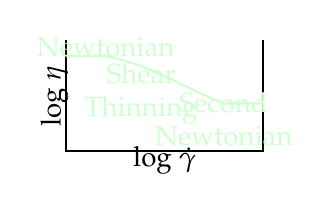
\begin{tikzpicture}[scale=0.5, yscale=0.8]
			% Shear rate vs viscosity
			\draw[-,thick] (0,3.5) -- (0,0) -- (5,0) -- (5,3.5);
			\node at (2.5,-0.3) {log $\dot{\gamma}$};
			\node[rotate=90] at (-0.3,1.75) {log $\eta$};

			% Flow curve
			\draw[g3,thick] (0,3) -- (1,3)
			.. controls (2,2.8) and (3,2) .. (4,1.5)
			-- (5,1.5);

			% Regions
			\node[g3, align=center] at (1,3.3) {Newtonian};
			\node[g3, align=center] at (1.9,1.8) {Shear\\Thinning};
			\node[g3, align=center] at (4,1) {Second\\Newtonian};
		\end{tikzpicture}
	\end{minipage}
	\hfill
	\begin{minipage}{0.49\textwidth}
		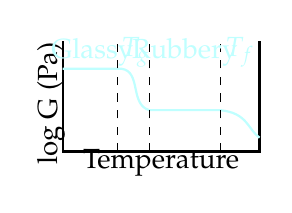
\begin{tikzpicture}[scale=0.5, yscale=0.7]
			% Axes
			\draw[-,thick] (0,4) -- (0,0) -- (5,0) -- (5,4);
			\node at (2.5,-0.4) {Temperature};
			\node[rotate=90] at (-0.3,1.75) {log G (Pa)};

			% Modulus curve: Glassy plateau -> Tg drop -> Rubbery plateau -> Flow
			\draw[b3,thick]
			(0,3) -- (1.5,3) % Glassy plateau
			.. controls (2,2.9) and (1.7,1.7) .. (2.2,1.5) % Drop through Tg region
			-- (4,1.5) % Rubbery plateau
			.. controls (4.7,1.4) and (4.7,0.8) .. (5,0.5); % Drop into flow region

			% Dashed lines (Positions remain unchanged)
			\draw[dashed] (1.4,0) -- (1.4,4);
			\draw[dashed] (2.2,0) -- (2.2,4);
			\draw[dashed] (4,0) -- (4,4);

			% Regions and labels
			\node[b3] at (0.75,3.6) {Glassy};
			\node[b3] at (1.85,3.6) {$T_g$};
			\node[b3] at (3.1,3.6) {Rubbery};
			\node[b3] at (4.5,3.6) {$T_f$};
		\end{tikzpicture}
	\end{minipage}\\
	\nc[v3]{Processing}\\
	\textbf{Capillary Rheometer:} \(\dot{\gamma} = \frac{4Q}{\pi R^3}, \quad \tau = \frac{(P_0 - P_L)R}{2L}\)\\

	\(\dot{\gamma}\) = shear rate, \(Q\) = volumetric flow rate, \(R\) = die radius, \(L\) = die length, and \((P_0 - P_L)\) = pressure drop.\\[-0.6em]

	\textbf{Rotational Rheometer – Cone \& Plate:}\\[-0.8em]

	\(\dot{\gamma} = \frac{\Omega}{\theta_0}, \quad \tau = \frac{3T}{2\pi R^3}, \quad \eta = \frac{\tau}{\dot{\gamma}} = \frac{3T\theta_0}{2\pi R^3 \Omega}\)\\

	\(\Omega\) = angular velocity, \(\theta_0\) = cone angle, \(T\) = torque, \(R\) = plate radius.\\

	\textbf{Rotational Rheometer – Parallel Plates:}\\[-0.8em]

	\(\dot{\gamma} = \frac{r\Omega}{H}, \quad \tau = \frac{3T}{2\pi R^3}, \quad \eta = \frac{\tau}{\dot{\gamma}} = \frac{3TH}{2\pi R^3 r \Omega}\)\\[-0.3em]

	\(r\) = radial position, \(H\) = gap height.\\[-0.5em]

	\textbf{Gibbs Free Energy for Blends:}\\
	\(\Delta G = \Delta H - T \Delta S, \quad \Delta H = \nu(\delta_1 - \delta_2)^2 \phi_1 \phi_2\)\\
	\(\nu\) = molar volume, \(\delta\) = solubility parameters, \(\phi\) = volume fractions.\\[-1em]

	\textbf{Melt Flow Index (MFI):} Mass of polymer extruded under standard conditions \([g/10 \, \text{min}]\)

\end{conceptbox}

\begin{conceptbox}[r1]{Dimensional Analysis}


	\textbf{Buckingham Pi Theorem:} Every system with m physical quantities reduced to m-n dimensionless groups, n = number basic dimensions\\

	\textbf{Basic Dimensions [MLT$\Theta$]:}\\
	\begin{minipage}{0.95\textwidth}
		\tiny
		\noindent
		\begin{tabular}{cccc}
			Length (L): m & %
			Mass (M): kg  & %
			Time (T): s   & %
			Temp ($\Theta$): K
		\end{tabular}
	\end{minipage}\\

	\textbf{Matrix Method:}
	(1) Select n dimension core matrix (repeating vars)\\
	(2) Form [L,M,T] rows x vars cols matrix\\
	(3) Solve for Pi groups: $\Pi_1 = f(\Pi_2, \Pi_3, ...)$\\

	\textbf{Key Dimensionless Numbers:}\\
	Deborah Number: De = $\frac{\text{Material relax time}}{\text{Process time}}$\\
	De $\to$ 0: Viscous fluid, De $\to$ $\infty$: Elastic solid\\

	Biot Number: Bi = $\frac{\text{Surface convection}}{\text{Internal conduction}}$ = $\frac{hL}{k}$\\

	Bi $\ll$ 1: Tc $\approx$ Ts (uniform temp)\\

	Bi $\gg$ 1: Ts $\approx$ T$_\infty$ (surface controlled)\\

	\begin{minipage}[t]{0.48\linewidth}
		\textbf{Scaling Laws:}\\
		Length: L $\propto$ size\\
		Area: A $\propto$ L$^2$\\
		Volume/Weight: V,W $\propto$ L$^3$\\
		Stress: $\sigma$ = W/A $\propto$ L
	\end{minipage}
	\hfill
	\begin{minipage}[t]{0.48\linewidth}
		\textbf{Similarity Types:}\\
		Geometric: shape ratios same\\
		Kinematic: velocity ratios same\\
		Dynamic: force ratios same
	\end{minipage}\\[-1em]
	\begin{center}
		\nc[r1]{\textbf{Matrix Transformation Method Example}}\\
	\end{center}
	\vspace{-1em}

	Consider pipe flow with pressure drop ($\Delta p$), diameter ($D$), length ($L$), viscosity ($\eta$), density ($\rho$), velocity ($u$)\\

	\textbf{Step 1: List Variables with Dimensions}\\[-1.25em]
	\begin{minipage}{0.48\textwidth}
		\begin{equation*}
			\begin{array}{c|c}
				\text{Variable} & \text{Dimension} \\
				\hline
				D               & L                \\
				\rho            & ML^{-3}          \\
				u               & LT^{-1}          \\
			\end{array}
		\end{equation*}
	\end{minipage}
	\hfill
	\begin{minipage}{0.48\textwidth}
		\begin{equation*}
			\begin{array}{c|c}
				\text{Variable} & \text{Dimension} \\
				\hline
				\Delta p        & ML^{-1}T^{-2}    \\
				L               & L                \\
				\eta            & ML^{-1}T^{-1}    \\
			\end{array}
		\end{equation*}
	\end{minipage}\\[0.5em]

	\textbf{Step 2: Select Core Matrix} (n=3 basic dimensions)\\
	Choose $D$, $\rho$, $u$ as repeating variables\\

	\textbf{Step 3: Form Dimensional Matrix}\\
	\begin{equation*}
		\begin{array}{c|ccc|ccc}
			  & D & \rho & u  & \Delta p & L & \eta \\
			\hline
			L & 1 & -3   & 1  & -1       & 1 & -1   \\
			M & 0 & 1    & 0  & 1        & 0 & 1    \\
			T & 0 & 0    & -1 & -2       & 0 & -1
		\end{array}
	\end{equation*}
	\textbf{Step 4: Solve for $\Pi$ Groups}\\
	\begin{minipage}{0.55\linewidth}
		For $\Pi_1$ using $\Delta p$: \\
		$[D^a \rho^b u^c \Delta p]=[M^0L^0T^0]$\\[-2em]
		\begin{align*}
			L:\quad & a - 3b + c - 1 = 0 \\
			M:\quad & b + 1 = 0          \\
			T:\quad & -c - 2 = 0
		\end{align*}
		Solving gives: $\Pi_1 = \frac{\Delta p}{\rho u^2}$\\
	\end{minipage}
	\hfill
	\begin{minipage}{0.44\linewidth}
		Similarly for remaining groups:\\[-2.5em]
		\begin{align*}
			\Pi_2 & = \frac{L}{D}                         \\
			\Pi_3 & = \frac{\eta}{D\rho u} = \frac{1}{Re}
		\end{align*}\\[-1.5em]
		\textbf{Final Result:}\\[0.5em]
		$f(\frac{\Delta p}{\rho u^2}, \frac{L}{D}, \frac{\eta}{D\rho u}) = 0$
	\end{minipage}\\
\end{conceptbox}
\vspace{-2em}
\begin{conceptbox}[o1]{Design of Experiments}
	\begin{minipage}{0.52\textwidth}
		\textbf{Seven-Step Process:}\\
		1. Identify Factors/Metrics\\
		2. Formulate Objective\\
		3. Design Experiment\\
		4. Run Trials\\
		5. Analyze Results\\
		6. Select Setpoints\\
		7. Iterate/Validate\\
	\end{minipage}
	\hfill
	\begin{minipage}{0.48\textwidth}
		\textbf{Control Factors:}\\
		Temperature, Pressure, Time\\
		Material Properties, Geometry\\
		Process Parameters\\
		\textbf{Noise Factors:}\\
		Manufacturing Variance\\
		Environmental Conditions\\
		User/Operation Variations\\
	\end{minipage}

	\textbf{Signal-to-Noise Ratio Analysis}
	{\color{v1}Signal-to-Noise Ratio (SNR)} measures the relationship between {\color{r1}response values} and their variation across {\color{b1}sample size}.\\
	\begin{minipage}{0.4\textwidth}
		\vspace{0.5em}
		\tiny
		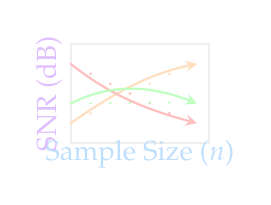
\begin{tikzpicture}[scale=0.5]
			% Axes
			\draw[thick, w] (0,0) rectangle (3.5,2.5);
			\node[inner sep=3pt] at (1.75,-0.3) {{\color{b1}Sample Size ($n$)}};
			\node[above, inner sep=3pt, rotate=90] at (0, 1.25) {{\color{v1}SNR (dB)}};

			% Larger-the-better curve
			\draw[-stealth, o1, thick] (0,0.5) .. controls (1,1.2) and (2,1.8) .. (3.2,2);
			\foreach \x in {0, 0.5, 1, 1.5, 2, 2.5, 3} {
					\fill[o1] (\x, {0.5 + 0.5*\x}) circle (1pt);
				}

			% Smaller-the-better curve
			\draw[-stealth, r1, thick] (0,2) .. controls (1,1.2) and (2,0.8) .. (3.2,0.5);
			\foreach \x in {0, 0.5, 1, 1.5, 2, 2.5, 3} {
					\fill[r1] (\x, {2 - 0.5*\x}) circle (1pt);
				}

			% Nominal-the-best curve
			\draw[-stealth, g1, thick] (0,1) .. controls (1,1.5) and (2,1.5) .. (3.2,1);
			\foreach \x in {0, 0.5, 1, 1.5, 2, 2.5, 3} {
					\fill[g1] (\x, {1 + 0.2*sin(3.14*\x)}) circle (1pt);
				}
		\end{tikzpicture}
	\end{minipage}
	\hfill
	\begin{minipage}{0.6\textwidth}
		\tiny
		\({\color{o1}\eta_L} = -10\log_{10}\left(\frac{1}{{\color{b1}n}}\sum_{i=1}^{{\color{b1}n}}\frac{1}{{\color{r1}y_i^2}}\right)\)\\[0.8em]

		\({\color{r1}\eta_S} = -10\log_{10}\left(\frac{1}{{\color{b1}n}}\sum_{i=1}^{{\color{b1}n}}{\color{r1}y_i^2}\right)\)\\[0.6em]

		\({\color{g1}\eta_N} = 10\log_{10}\left(\frac{{\color{r1}\bar{y}^2}}{s^2}\right)\)\\
	\end{minipage}\\
	\textbf{L9 Orthogonal Array} Experimental design matrix enabling efficient study of multiple factor effects with minimal trials.\\[-1em]
	\begin{minipage}{0.48\textwidth}
		\tiny
		\[%
			\begin{array}{c|cccc}%
				\text{} & {\color{o3}A} & {\color{g3}B} & {\color{b3}C} & {\color{v2}D} \\
				\hline
				1       & {\color{o3}1} & {\color{g3}1} & {\color{b3}1} & {\color{v2}1} \\
				2       & {\color{o3}1} & {\color{g3}2} & {\color{b3}2} & {\color{v2}2} \\
				3       & {\color{o3}1} & {\color{g3}3} & {\color{b3}3} & {\color{v2}3} \\
				4       & {\color{o3}2} & {\color{g3}1} & {\color{b3}2} & {\color{v2}3} \\
				5       & {\color{o3}2} & {\color{g3}2} & {\color{b3}3} & {\color{v2}1} \\
				6       & {\color{o3}2} & {\color{g3}3} & {\color{b3}1} & {\color{v2}2} \\
				7       & {\color{o3}3} & {\color{g3}1} & {\color{b3}3} & {\color{v2}2} \\
				8       & {\color{o3}3} & {\color{g3}2} & {\color{b3}1} & {\color{v2}3} \\
				9       & {\color{o3}3} & {\color{g3}3} & {\color{b3}2} & {\color{v2}1}
			\end{array}\\
		\]\\
	\end{minipage}
	\hfill
	\begin{minipage}{0.44\textwidth}
		\tiny
		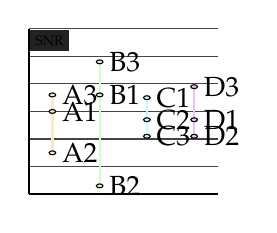
\begin{tikzpicture}[xscale=0.6, yscale=0.35] % Reduced scale
			% Background grid (subtle)
			\foreach \y in {1,...,6} {
					\draw[g] (0,\y) -- (4,\y);
				}

			% Axes
			\draw[thick, -] (0,0) -- (4,0);
			\draw[thick, -] (0,0) -- (0,6) node[below right, fill=b, inner sep=2pt] {\tiny SNR};

			% Factor A (Melt Temp)
			\draw[o3,thick] (0.5,1.5) -- (0.5,3.6);
			\draw[fill=o3] (0.5,1.5) circle (2pt) node[right] {A2};
			\draw[fill=o3] (0.5,3) circle (2pt) node[right] {A1};
			\draw[fill=o3] (0.5,3.6) circle (2pt) node[right] {A3};

			% Factor B (Shot Size)
			\draw[g3,thick] (1.5,0.3) -- (1.5,4.8);
			\draw[fill=g3] (1.5,0.3) circle (2pt) node[right] {B2};
			\draw[fill=g3] (1.5,3.6) circle (2pt) node[right] {B1};
			\draw[fill=g3] (1.5,4.8) circle (2pt) node[right] {B3};

			% Factor C (SCF Level)
			\draw[b3,thick] (2.5,2.1) -- (2.5,3.5);
			\draw[fill=b3] (2.5,2.1) circle (2pt) node[right] {C3};
			\draw[fill=b3] (2.5,2.7) circle (2pt) node[right] {C2};
			\draw[fill=b3] (2.5,3.5) circle (2pt) node[right] {C1};

			% Factor D (Inj. Speed)
			\draw[v2,thick] (3.5,2.1) -- (3.5,3.9);
			\draw[fill=v2] (3.5,2.1) circle (2pt) node[right] {D2};
			\draw[fill=v2] (3.5,2.7) circle (2pt) node[right] {D1};
			\draw[fill=v2] (3.5,3.9) circle (2pt) node[right] {D3};
		\end{tikzpicture}
	\end{minipage}\\[-1.2em]
	\textbf{Response Surface Analysis} Maps relationship between {\color{b1}input factors} and {\color{r1}system response} for {\color{g1}optimization}.\\

	\(
	{\color{r1}y} = {\color{v1}\beta_0} + \sum_{i=1}^{k}{\color{v1}\beta_i}{\color{b1}x_i} + \sum_{i=1}^{k}{\color{v1}\beta_{ii}}{\color{b1}x_i^2} + \sum_{i<j}^{k}{\color{v1}\beta_{ij}}{\color{b1}x_ix_j} + {\color{v1}\varepsilon}
	\)\\
	\begin{center}
		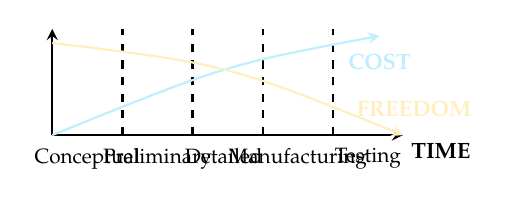
\begin{tikzpicture}[>=stealth,thick,scale=0.45, xscale=1.1]

			\draw[->] (0,0) -- (9,0) node[below right, scale=0.8]{\textbf{TIME}};
			\draw[->] (0,0) -- (0,3);

			\foreach \x in {1.8, 3.6, 5.4, 7.2} {
					\draw[dashed] (\x,0) -- (\x,3);
				}

			\node[below,yshift=-2pt, scale=0.75] at (0.9,0) {Conceptual};
			\node[below,yshift=-2pt, scale=0.75] at (2.7,0) {Preliminary};
			\node[below,yshift=-2pt, scale=0.75] at (4.4,0) {Detailed};
			\node[below,yshift=-2pt, scale=0.75] at (6.3,0) {Manufacturing};
			\node[below,yshift=-2pt, scale=0.75] at (8.1,0) {Testing};

			\draw[-stealth, b2,thick] (0,0) .. controls (4.5,2) .. (8.4,2.8) node[below, inner sep =8pt, scale=0.8]{\textbf{COST}};

			\draw[-stealth, o2,thick] (0,2.6) .. controls (4.5,2) .. (9,0) node[above, inner sep =8pt, scale=0.8]{\textbf{\quad FREEDOM}};

		\end{tikzpicture}
	\end{center}
\end{conceptbox}
\begin{conceptbox}[b1]{Continuity}

	\nc[r2]{Mass Conservation}\\

	\begin{minipage}{\linewidth}
		\textbf{Cartesian:} \\

		\(\frac{\partial u_x}{\partial x} + \frac{\partial u_y}{\partial y} + \frac{\partial u_z}{\partial z} = 0\)\\

		\textbf{Cylindrical:}\\

		\(\frac{1}{r}\frac{\partial}{\partial r}(rv_r) + \frac{1}{r}\frac{\partial v_\theta}{\partial \theta} + \frac{\partial v_z}{\partial z} = 0\)\\
		\vspace{5pt}
		\tdplotsetmaincoords{75}{160}
		\begin{tikzpicture}[overlay]
			\node[anchor=east, inner sep = 5pt] at (1.02\linewidth,0.7) {
				\begin{tikzpicture}[
						font = \tiny \boldmath,
						tdplot_main_coords,
						anchor=center,
						inner sep = 3pt,
						axis/.style={->,blue,line width=0.8pt},
						cube/.style={},
						scale=0.75,
						% Define common styles
						face/.style={cube,line width=0.6pt,draw=w},
						filled face/.style={face,fill=b!90,opacity=0.8},
						arrow style/.style={-stealth,line width=0.5pt},
					]

					% Define coordinate ranges
					\def\gridrange{1.7,2.07,2.43,2.8}
					\def\zrange{0.2,0.57,0.93,1.3}

					% Coordinate system
					\begin{scope}[shift={(-0.2,0,-1.5)}, scale=0.8]
						\draw[-stealth] (0,0,0) -- (0.5,0,0) node[scale=0.9, anchor=east] {x};
						\draw[-stealth] (0,0,0) -- (0,0.7,0) node[scale=0.9, anchor=north east] {y};
						\draw[-stealth] (0,0,0) -- (0,0,0.4) node[scale=0.9, anchor=south] {z};
					\end{scope}

					% Base planes
					\draw[cube, fill=b2, opacity=.5] (1.5,1.5,-0.3) -- (3,1.5,-0.3) -- (3,3,-0.3) -- (1.5,3,-0.3) -- cycle;
					\draw[cube,thick,draw=b2] (1.5,1.5,-0.3) -- (3,1.5,-0.3) -- (3,3,-0.3) -- (1.5,3,-0.3) -- cycle;

					% Side planes
					\begin{scope}[opacity=0.8]
						\draw[cube, fill=b] (1.1,1.5,0) -- (1.1,3,0) -- (1.1,3,1.5) -- (1.1,1.5,1.5) -- cycle;
						\draw[cube, fill=r2!90, opacity=.4] (1.1,1.5,0) -- (1.1,3,0) -- (1.1,3,1.5) -- (1.1,1.5,1.5) -- cycle;
						\draw[cube,thick,draw=r2] (1.1,1.5,0) -- (1.1,3,0) -- (1.1,3,1.5) -- (1.1,1.5,1.5) -- cycle;
					\end{scope}

					% Main cube faces
					\draw[cube, fill=b, draw=b] (1.5,1.5,0) -- (1.5,3,0) -- (1.5,3,1.5) -- (1.5,1.5,1.5) -- cycle;

					% Inner faces with opacity
					\foreach \face in {
							{(1.5,1.5,0) -- (3,1.5,0) -- (3,1.5,1.5) -- (1.5,1.5,1.5)},
							{(1.5,1.5,0) -- (1.5,3,0) -- (1.5,3,1.5) -- (1.5,1.5,1.5)},
							{(1.5,1.5,0) -- (1.5,3,0) -- (3,3,0) -- (3,1.5,0)}
						} {
							\draw[cube,thick,draw=w, fill=b!90] \face;
						}

					% Arrows in YZ plane
					\foreach \y in \gridrange {
						\foreach \z in \zrange {
							\draw[arrow style, r2, opacity=((\y-1.4)/1.5 + (\z+0.5)/1.5)/2]
							(0.6,\y,\z) -- (3.6,\y,\z);
						}
					}

					% Vertical arrows
					\foreach \x in \gridrange {
						\foreach \y in \gridrange {
							\draw[arrow style, b2, opacity={((\y-1.7)/1.1 + (\x-1.7)/1.1)/2}]
							(\x,\y,-0.7) -- (\x,\y,2);
						}
					}

					% Outer faces
					\foreach \face in {
							{(1.5,3,0) -- (3,3,0) -- (3,3,1.5) -- (1.5,3,1.5)},
							{(1.5,1.5,1.5) -- (1.5,3,1.5) -- (3,3,1.5) -- (3,1.5,1.5)},
							{(3,1.5,0) -- (3,3,0) -- (3,3,1.5) -- (3,1.5,1.5)}
						} {
							\draw[filled face] \face;
							\draw[face] \face;
						}

					% Final arrow set with gradient
					\foreach \x in \gridrange {
						\foreach \y in \gridrange {
							\draw[arrow style, draw=b2,
								opacity={((\y-1.5)/1.1 + (\x-1.6)/1.1)/2.1}]
							(\x,\y,1.5) -- (\x,\y,2);
						}
					}
					\foreach \y in \gridrange {
						\foreach \z in \zrange {
							\draw[arrow style, draw=r2,
								opacity={((\y-1.5)/1.1 + (\z-0.1)/1.1)/2.1}]
							(3,\y,\z) -- (3.6,\y,\z);
						}
					}

					\begin{scope}[canvas is xz plane at y=2.25]
						\node[scale=1.1, text=r2, inner sep=2pt, xscale=-1, transform shape] at (0.2,0.65) {$u_x\Delta y\Delta z$};
					\end{scope}

					\begin{scope}[canvas is xz plane at y=2.25]
						\node[scale=1.1, text=r2, inner sep=2pt, xscale=-1, transform shape] at (4.2,1.8) {$(u_x+\Delta u_x)\Delta y\Delta z$};
					\end{scope}

					\begin{scope}[canvas is xz plane at y=3]
						\node[scale=1.1, text=b2,fill=b, inner sep=1pt, xscale=-1, transform shape] at (2.27,-0.5) {$u_y\Delta x\Delta z$};
					\end{scope}

					\begin{scope}[canvas is xz plane at y=2.25]
						\node[scale=1.1, text=b2, inner sep=2pt,  xscale=-1, transform shape] at (2.25,2.25) {$(u_y+\Delta u_y)\Delta x\Delta z$};
					\end{scope}
				\end{tikzpicture}
			};
		\end{tikzpicture}
	\end{minipage}
	\textbf{Mass Flow Rate:} \(\dot{m} = \rho Q = \rho \mathbf{u} \cdot \mathbf{A}\)\\

	\textbf{Continuity (Incompressible):} \(\nabla \cdot \mathbf{u} = 0\)\\

	\textbf{Continuity (Compressible):} $\frac{\partial}{\partial x} (\rho u_x) + \frac{\partial}{\partial y} (\rho u_y) + \frac{\partial}{\partial z} (\rho u_z) = 0$\\

	\nc[b3]{Momentum Conservation}


	$\rho \left( \frac{\partial u_x}{\partial t} + u_x \frac{\partial u_x}{\partial x} + u_y \frac{\partial u_x}{\partial y} + u_z \frac{\partial u_x}{\partial z} \right)$ \\

	\quad\quad $= -\frac{\partial p}{\partial x} + \mu \left( \frac{\partial^2 u_x}{\partial x^2} + \frac{\partial^2 u_x}{\partial y^2} + \frac{\partial^2 u_x}{\partial z^2} \right) + \rho g_x$ \\


	\(\rho\frac{D\mathbf{u}}{Dt} = -\nabla p + \eta\nabla^2\mathbf{u} + \rho\mathbf{g}\)\\[0.4em]

	\textbf{Non-Newtonian Viscosity:}\\

	\(\eta = \eta(\dot{\gamma}) = \eta\left(\sqrt{\frac{1}{2}\sum_{i,j}\left(\frac{\partial u_i}{\partial x_j} + \frac{\partial u_j}{\partial x_i}\right)^2}\right)\)\\

	\nc[y1]{Energy Conservation}
	\tiny
	$\rho c_v \left( \frac{\partial T}{\partial t} + u_x \frac{\partial T}{\partial x} + u_y \frac{\partial T}{\partial y} + u_z \frac{\partial T}{\partial z} \right)$ \\

	$=k \left( \frac{\partial^2 T}{\partial x^2} + \frac{\partial^2 T}{\partial y^2} + \frac{\partial^2 T}{\partial z^2} \right) + 2\mu \left( \left( \frac{\partial v_x}{\partial x} \right)^2 + \left( \frac{\partial v_y}{\partial y} \right)^2 + \left( \frac{\partial v_z}{\partial z} \right)^2 \right)$ \\
	$\quad + \mu \left( \left( \frac{\partial v_x}{\partial y} + \frac{\partial v_y}{\partial x} \right)^2
		+ \left( \frac{\partial v_x}{\partial z} + \frac{\partial v_z}{\partial x} \right)^2 \right) + \left. \left( \frac{\partial v_y}{\partial z} + \frac{\partial v_z}{\partial y} \right)^2 \right) + \dot{Q}$\\ \ssmall

	\(\rho C_p \frac{DT}{Dt} = -\nabla \cdot \mathbf{q} + \dot{Q} + \dot{Q}_\text{viscous heating}\)\\[0.3em]
	\begin{minipage}{0.49\textwidth}
		\textbf{Material Derivative:}\\[0.4em]
		\(\frac{DT}{Dt} = \frac{\partial T}{\partial t} + \mathbf{u} \cdot \nabla T\)
	\end{minipage}
	\hfill
	\begin{minipage}{0.49\textwidth}
		\textbf{Fourier's Law:}\\
		\(\mathbf{q} = -k\nabla T\)
	\end{minipage}\\[0.4em]

	\textbf{Heat Conduction:}\\
	\(-\nabla \cdot \mathbf{q} = k\nabla^2T = k\left(\frac{\partial^2 T}{\partial x^2} + \frac{\partial^2 T}{\partial y^2} + \frac{\partial^2 T}{\partial z^2}\right)\)\\

	\textbf{Simple Shear Heating:} \(\dot{Q}_\text{viscous heating} = \eta\left(\frac{\partial u}{\partial y}\right)^2\)\\
	\\
	\\
	\\
	\\
	\columnbreak
	\nc[b1]{Order of Magnitude}\\
	\begin{minipage}{\textwidth}
		From continuity: \((U/L_x) \sim (V/L_y)\). If \(L_x \gg L_y\), then \(U \gg V\).\\[0.4em]
		Momentum in \(x\)-dir: \(\rho U^2/L_x \sim \Delta p/L_x \sim \mu U/L_x^2 \sim \mu U/L_y^2\).\\[0.4em]
		Dominance depends on \(\frac{L_x}{L_y}\) and \(\text{Re}=\frac{\rho U L_x}{\mu}\). For small Re and large \(L_x/L_y\), viscous terms \((\mu U/L_y^2)\) dominate over inertial \((\rho U^2/L_x)\).\\[0.4em]
		Second derivative: \(\partial^2 u/\partial x^2 \sim U/L_x^2\) vs. squared gradient: \((\partial u/\partial x)^2 \sim (U/L_x)^2\). Scaling guides term retention.\\

	\begin{minipage}{0.48\textwidth}
		\textbf{Geometric Parameters:}\\
		\textbf{Width Ratio:} \\
		$ \frac{W}{L} \sim O(1) $\\
		\textbf{Channel Aspect:} \\
		$ \frac{h}{W} \ll 1 $\\
		\textbf{Flow Analysis:}\\
		\textbf{Continuity Scaling:} \\
		$ \frac{U}{L_x} \sim \frac{V}{L_y} $\\
		\textbf{Momentum Scaling:} \\
		$ \rho \frac{U^2}{L_x} \sim \frac{\Delta P}{L_x} \sim \mu \frac{U}{L_y^2} $
	\end{minipage}
	\hfill
	\begin{minipage}{0.48\textwidth}
		\textbf{Critical Numbers:}\\
		\textbf{Re}$\left(\frac{L_y}{L_x}\right)$ \\
		\textbf{Re}$\left(\frac{L_y}{L_x}\right)$\\
		\textbf{Process-Specific Scaling:}\\
		\textbf{Injection Molding:} \\
		$ Re \ll 1, \quad \epsilon \ll 1 $\\
		\textbf{Film Casting:} \\
		$ We = \frac{\rho v^2 h}{\sigma} \gg 1 $
	\end{minipage}
	\end{minipage}

\end{conceptbox}

\begin{conceptbox}[b3]{Solving the Governing Equations}
	\nc[b3]{Fundamental Assumptions and Reductions}\\[-1.7em]
	\begin{center}
		\tiny
		\renewcommand{\arraystretch}{1.2} % Adjust vertical padding
		\begin{tabular}{|p{0.35\textwidth}|p{0.48\textwidth}|}
			\hline
			\textbf{Assumption / Approach} & \textbf{Resulting Simplification} \\[0.2em]
			\hline
			Steady State: $\frac{\partial}{\partial t}=0$ & {\color{r1}$\cancel{\frac{\partial \rho}{\partial t}} + \nabla \cdot (\rho \mathbf{u}) = 0$} \\
			& {\color{b3}$\rho \cancel{\frac{\partial \mathbf{u}}{\partial t}} + \rho (\mathbf{u} \cdot \nabla) \mathbf{u} = -\nabla p + \mu \nabla^2 \mathbf{u}$} \\[0.2em]
			\hline
			Constant Material Properties: $\rho = \text{const}, \mu = \text{const}$ & {\color{r1}$\frac{\partial \rho}{\partial t} = 0, \; \frac{\partial \rho}{\partial x_i} = 0$} \\
			& {\color{r1}$\implies \nabla \cdot \mathbf{u} = 0$} \\[0.2em]
			\hline
			Fully Developed Flow: $\frac{\partial u_x}{\partial x} = 0$ & {\color{r1}$\cancel{\frac{\partial u_x}{\partial x}} + \frac{\partial u_y}{\partial y} + \frac{\partial u_z}{\partial z} = 0$} \\[0.2em]
			\hline
			Dimensions of Geometry: $\frac{\partial}{\partial z} = 0, \; u_z = 0$ & {\color{r1}$\frac{\partial u_x}{\partial x} + \frac{\partial u_y}{\partial y} + \cancel{\frac{\partial u_z}{\partial z}} = 0$ with $\cancel{u_z} = 0$} \\[0.2em]
			\hline
			Symmetry (Independent of Width): $\frac{\partial}{\partial z} = 0$ & {\color{r1}$\frac{\partial u_x}{\partial x} + \frac{\partial u_y}{\partial y} + \cancel{\frac{\partial u_z}{\partial z}} = 0$} \\[0.2em]
			\hline
			Dimensional Analysis (Low Re) & {\color{b3}$\rho (\mathbf{u} \cdot \nabla) \mathbf{u} = \cancel{\rho (\mathbf{u} \cdot \nabla) \mathbf{u}} = 0 \implies 0 = -\nabla p + \mu \nabla^2 \mathbf{u}$} \\[0.2em]
			\hline
			Constant Material Properties (Reiterated) & {\color{r1}$\nabla \cdot \mathbf{u} = 0$}, {\color{b3}$0 = -\nabla p + \mu \nabla^2 \mathbf{u}$} \\[0.2em]
			\hline
			Lubrication Approximation: $\frac{\partial p}{\partial x} \gg \frac{\partial p}{\partial y}$ & {\color{b3}$-\nabla p = -\frac{\partial p}{\partial x} \hat{i} - \cancel{\frac{\partial p}{\partial y}} \hat{j}$} \\[0.2em]
			\hline
		\end{tabular}
		\ssmall
	\end{center}
	\vspace{-1em}

	\nc[b3]{Lubrication}\\
	\begin{minipage}{0.48\textwidth}
		\textbf{Key Parameters:} \\
		$ \epsilon = \frac{h}{L} \ll 1 \quad (\text{thin film}) $ \\
		$ Re = \frac{\rho U h}{\mu}$

		\textbf{Simplified Momentum:} \\
		$ \frac{\partial^2 u}{\partial y^2} = \frac{1}{\mu}\frac{\partial p}{\partial x} $
	\end{minipage}
	\hfill
	\begin{minipage}{0.48\textwidth}
		\textbf{Velocity Profile:} \\
		$ u(y) = \frac{1}{2\mu}\left(\frac{dp}{dx}\right)(y^2 - hy) $\\

		\textbf{Flow Rate:} \\
		$ q = -\frac{h^3}{12\mu}\left(\frac{dp}{dx}\right) $
	\end{minipage}
			\nc[b1]{Scale Analysis and Term Reduction}\\
		\textbf{Inertial terms:} \(\rho U \frac{U}{L_x} \approx \rho V \frac{U}{L_y}\quad\quad\quad\quad\)\textbf{Viscous terms:} \(\mu \frac{U}{L_y^2}\)
	Here, \(U\) and \(V\) are the velocities in the \(x\) and \(y\) directions, respectively. \(L_x\) and \(L_y\) are the lengths in the \(x\) and \(y\) directions. \(\rho\) is the fluid density, and \(\mu\) is the dynamic viscosity.\\

	\begin{minipage}{0.62\textwidth}
		To see which terms are more important, we use the Reynolds number (\(Re\))\\

		\( Re = \frac{\rho U L_y}{\mu} \)\\

		If \(Re \frac{L_y}{L_x} \ll 1\), viscous forces are more significant than inertial forces.
	\end{minipage}
	\begin{minipage}{0.3\textwidth}
		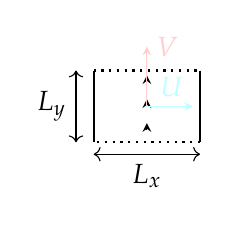
\begin{tikzpicture}[scale=0.45, yscale=0.675]
			% Draw main cavity (cut section)
			\draw[thick] (0,0) -- (0,3);
			\draw[dotted, thick] (0,3) -- (3,3);
			\draw[thick] (3,3) -- (3,0);
			\draw[dotted, thick] (3,0) -- (0,0);

			% Add dimensions
			\draw[<->] (-0.5,0) -- (-0.5,3) node[midway,left] {$L_y$};
			\draw[<->] (0,-0.5) -- (3,-0.5) node[midway,below] {$L_x$};

			% Add flow arrows
			\foreach \y in {0.5,1.5,2.5} {
					\draw[-stealth] (1.5,\y) -- (1.5,\y+0.3);
				}

			% Label velocity components
			\draw[-stealth,r3] (1.5,1.5) -- (1.5,4) node[right] {$V$};
			\draw[-stealth,b3] (1.5,1.5) -- (2.8,1.5) node[above left] {$U$};
		\end{tikzpicture}
	\end{minipage}\\
\end{conceptbox}
	\pagebreak
\begin{conceptbox}[v1]{Textbook}
	\tiny
	\nc[v1]{Example 9.1: Flow in a tube}

Consider the classical problem of pressure drop during flow in a smooth straight pipe, ignoring the inlet effects. The first step is to list all possible variables or quantities that are related to the problem under consideration. In this case, we have:\\

\textbf{Target quantity:} Pressure drop $\Delta p$\\
\textbf{Geometric variables:} Pipe diameter $D$, and pipe length $L$\\
\textbf{Physical or material properties:} viscosity $\eta$, density $\rho$\\
\textbf{Process variable:} average fluid velocity $u$\\

If we choose $D$, $u$, and $\rho$ as the repeating variables, the dimensional matrix is written as:\\

\begin{equation}
\begin{array}{ccccccc}
    & D & u & \rho & \Delta p & L & \eta \\
M & 0 & 0 & 1 & 1 & 0 & 1 \\
L & 1 & 1 & -3 & -1 & 1 & -1 \\
T & 0 & -1 & 0 & -2 & 0 & -1
\end{array}
\end{equation}

After reducing the core matrix to an identity matrix, the dimensional matrix becomes:\\

\begin{equation}
\begin{array}{ccccccc}
    & D & u & \rho & \Delta p & L & \eta \\
M & 1 & 0 & 0 & 0 & 1 & 1 \\
L & 0 & 1 & 0 & 2 & 0 & 1 \\
T & 0 & 0 & 1 & 1 & 0 & 1
\end{array}
\tag{9.8}
\end{equation}

which results in the 3 dimensionless groups,\\

\begin{equation}
\Pi_1 = \frac{\Delta p}{u^2\rho} = Eu \text{ (Euler number)}
\tag{9.9}
\end{equation}
\begin{equation}
\Pi_2 = \frac{L}{D}
\end{equation}
\begin{equation}
\Pi_3 = \frac{\eta}{Du\rho} = Re^{-1} \text{ (Reynolds number)}
\end{equation}

The following relationship can be written:\\

\begin{equation}
f\left(Eu, Re, \frac{L}{D}\right) = 0
\tag{9.10}
\end{equation}

which, of course, by itself cannot produce the nature of the relation; however, the form of the function $f$ can be generated experimentally.\\

\nc[v1]{Dimensionless variables}\\
\tiny
	\centering
	\renewcommand{\arraystretch}{2.2} % Adjust vertical padding
		\begin{tabular}{|l|c|c|c|}
				\hline
				\textcolor{w}{Name} & \textcolor{w}{Symbol} & \textcolor{w}{Definition} & \textcolor{w}{Meaning} \\
				\hline
				
				Biot & $Bi$ & $\dfrac{hL}{k}$ & $\dfrac{\text{Convection}}{\text{Conduction}}$ \\
				\hline
				
				Brinkman & $Br$ & $\dfrac{\eta u^2}{k\Delta T}$ & $\dfrac{\text{Viscous}}{\text{Conduction}}$ \\
				\hline
				
				Capillary & $Ca$ & $\dfrac{\tau R}{\sigma_s}$ & $\dfrac{\text{Deviatoric}}{\text{Surface}}$ \\
				\hline
				
				Damköhler & $Da$ & $\dfrac{c\Delta H_r}{\rho C_p T_0}$ & $\dfrac{\text{Reaction}}{\text{Internal}}$ \\
				\hline
				
				Deborah & $De$ & $\dfrac{\lambda}{t}$ & $\dfrac{\text{Relaxation}}{\text{Process}}$ \\
				\hline
				
				Fourier & $Fo$ & $\dfrac{\alpha t}{L^2}$ & $\dfrac{\text{Process}}{\text{Thermal}}$ \\
				\hline
				
				Graetz & $Gz$ & $\dfrac{uL}{\alpha}\left(\dfrac{d}{L}\right)$ & $\dfrac{\text{Convection}}{\text{Conduction}}$ \\
				\hline
				
				Nusselt & $Nu$ & $\dfrac{hL}{k_{fluid}}$ & $\dfrac{\text{Convective}}{\text{Conductive}}$ \\
				\hline
				
				Péclet & $Pe$ & $\dfrac{UL}{\alpha}$ & $\dfrac{\text{Advection}}{\text{Diffusion}}$ \\
				\hline
				
				Prandtl & $Pr$ & $\dfrac{\nu}{\alpha}$ & $\dfrac{\text{Momentum}}{\text{Thermal}}$ \\
				\hline
				
				Reynolds & $Re$ & $\dfrac{\rho uL}{\eta}$ & $\dfrac{\text{Inertia}}{\text{Viscous}}$ \\
				\hline
				
				Schmidt & $Sc$ & $\dfrac{\nu}{D}$ & $\dfrac{\text{Mechanical}}{\text{Diffusion}}$ \\
				\hline
				
				Weissenberg & $We$ & $\lambda\dot{\gamma}$ or $\dfrac{N_1}{\tau}$ & $\dfrac{\text{Elastic}}{\text{Viscous}}$ \\
				\hline
				\end{tabular}
	
\end{conceptbox}
\columnbreak
\begin{conceptbox}[w]{examples}
	\tiny
	\nc[r3]{Pressure-Driven Flow Through Slit}

	\textbf{Assumptions}\\
	The following assumptions are made:\\
	1. The flow is steady, fully developed, and entrance effects are ignored.\\
	2. The fluid is Newtonian and incompressible.\\
	3. The flow is unidirectional, with only one non-zero velocity component \(u_z\).\\

	\textbf{Governing Equations}\\
	The continuity equation for an incompressible flow reduces to\\
	\(\frac{\partial u_z}{\partial z} = 0\).\\

	The \(z\)-momentum equation for a Newtonian, incompressible flow (Navier-Stokes equations) is given by\\
	\(-\frac{\partial p}{\partial z} + \mu \frac{\partial^2 u_z}{\partial y^2} = 0\).\\

	The \(x\)- and \(y\)-momentum components reduce to\\
	\(-\frac{\partial p}{\partial x} = -\frac{\partial p}{\partial y} = 0\).\\

	This indicates that the pressure depends only on \(z\). Since \(u_z\) does not vary with \(z\), the pressure gradient \(\frac{\partial p}{\partial z}\) is constant:\\
	\(\frac{\partial p}{\partial z} = \frac{\Delta p}{L}\).\\

	\textbf{Simplified Momentum Equation}\\
	Substituting the constant pressure gradient into the \(z\)-momentum equation:\\
	\(\frac{1}{\mu} \frac{\Delta p}{L} = \frac{\partial^2 u_z}{\partial y^2}\).\\

	\textbf{Boundary Conditions}\\
	No-slip boundary conditions are applied:\\
	\(u_z\left(\pm \frac{h}{2}\right) = 0\).\\

	\textbf{Solution for Velocity Profile}\\
	Integrating the simplified momentum equation twice and applying the boundary conditions, the velocity profile is obtained as\\
	\(u_z(y) = \frac{h^2}{8\mu} \frac{\Delta p}{L} \left[ 1 - \left( \frac{2y}{h} \right)^2 \right]\).\\

	\textbf{Mean Velocity}\\
	The mean velocity in the channel is calculated as\\
	\(\bar{u}_z = \frac{2}{h} \int_0^{h/2} u_z(y) \, dy = \frac{h^2}{12\mu} \frac{\Delta p}{L}\).\\

	\textbf{Volumetric Flow Rate}\\
	The volumetric flow rate is then given by\\
	\(Q = hW\bar{u}_z = \frac{Wh^3}{12\mu} \frac{\Delta p}{L}\),\\
	where \(W\) is the width of the channel.\\
	\tiny
	\nc[y3]{Shear Flow and Viscous Heating}

	\textbf{Assumptions}\\
	The following assumptions are made:\\
	1. The material is at \(210^\circ \text{C}\).\\
	2. The plate has a surface area of \(100 \, \text{cm}^2\) and is moving at a constant speed of \(u_w = 1.0 \, \text{cm/s}\).\\
	3. The gap between the plates is \(h = 0.1 \, \text{cm}\).\\
	4. The fluid follows the apparent shear viscosity (\(\eta_a = \mu\)) vs. shear rate (\(\dot{\gamma}\)) relationship provided.\\

	\textbf{Governing Equations}\\
	The viscous heating per unit volume is governed by the equation:\\
	\(\Phi_v = \mu \left( \frac{\partial u}{\partial y} \right)^2\),\\
	where:\\
	\(\Phi_v\) is the viscous heating per unit volume,\\
	\(\mu\) is the shear viscosity,\\
	\(\frac{\partial u}{\partial y}\) is the velocity gradient.\\

	\textbf{Shear Rate Calculation}\\
	The velocity gradient (shear rate) is given by:\\
	\(\dot{\gamma} = \frac{\partial u}{\partial y} = \frac{u_w}{h}\).\\
	Substituting the given values:\\
	\(\dot{\gamma} = \frac{1.0 \, \text{cm/s}}{0.1 \, \text{cm}} = 10 \, \text{s}^{-1}\).\\

	\textbf{Viscosity from Graph}\\
	From the given graph, the viscosity \(\mu\) corresponding to \(\dot{\gamma} = 10 \, \text{s}^{-1}\) is approximately:\\
	\(\mu = 0.2 \, \text{Pa}\cdot\text{s}\).\\

	\textbf{Viscous Heating Calculation}\\
	Substituting \(\mu\) and \(\dot{\gamma}\) into the viscous heating formula:\\
	\(\Phi_v = \mu \dot{\gamma}^2 = (0.2) (10)^2 = 20 \, \text{W/m}^3\).\\

	\textbf{Adiabatic Boundary Condition}\\
	With adiabatic boundaries, the heat generated internally is retained, leading to a uniform temperature rise throughout the fluid domain due to symmetry and constant thermal properties.

	\textbf{Conclusion on Temperature Rise}\\
	The temperature rise is uniform throughout the fluid domain due to the adiabatic boundary conditions and uniform generation of viscous heating.

	\nc[y3]{Viscous Heating}

	First, let's find $\mu$ from the plot and known parameters.

	\textbf{What is $\dot{\gamma}$ (shear rate)?}

	\[
	\dot{\gamma} = \frac{u_0}{h} = \frac{1.0 \, \text{(cm/sec)}}{0.1 \, \text{(cm)}} = 10 \, \text{sec}^{-1}
	\]

	Say, 
	\[
	\eta = 1.2 \times 10^5 \, \text{g/cm.sec}.
	\]

	Now let's simplify $\Phi_v$:

	\[
	\Phi_v = 2 \left[ \left(\frac{\partial u_x}{\partial x}\right)^2 + \left(\frac{\partial u_y}{\partial y}\right)^2 + \left(\frac{\partial u_z}{\partial z}\right)^2 \right] \quad \quad \quad \quad \quad \quad \quad \quad\]\\[-1em]
	\[ \quad \quad \quad \quad + 
	\left[ \left(\frac{\partial u_y}{\partial x} + \frac{\partial u_x}{\partial y} \right)^2
	+ 
	\left(\frac{\partial u_z}{\partial y} + \frac{\partial u_y}{\partial z}\right)^2 
	+ 
	\left(\frac{\partial u_x}{\partial z} + \frac{\partial u_z}{\partial x}\right)^2 \right].
	\]

	Only $u_x$ is not zero, and it is a function of $y$. 

	\[
	\Rightarrow \Phi_v = 2 \left( \frac{\partial u_x}{\partial y} \right)^2 \quad \Rightarrow \quad \Phi_v = 2 \left( \frac{u_0}{h} \right)^2 = 2 \times 10^2 \, \text{sec}^{-2}.
	\]

	\[
	\Rightarrow \mu \Phi_v = 1.2 \times 10^7 \, \left[ 1.2 \times 10^5 \times 2 \times 10^2 \right] \, \text{g/cm.sec}.
	\]

	\textbf{Units:}
	\[
	\text{Energy per unit time per unit volume: } \quad 
	\frac{\text{g.cm}}{\text{sec}^2} \cdot \frac{\text{cm}}{\text{sec}} \cdot \frac{1}{\text{cm}^3} 
	\]

	\nc[y3]{Uniform Temperature Rise}\\

	Since $\frac{\partial u_x}{\partial y}$ (or $\dot{\gamma}$) is uniform throughout the flow domain, so is the viscosity ($\mu$). Thus, $\mu \Phi_v$ should be uniform $\Rightarrow T$ is uniform.\\

	\nc[o3]{Flow Through Cylindrical Pipe}

	Tube flow is encountered in several polymer processes, such as in extrusion dies and sprue and runner systems inside injection molds. When deriving the equations for pressure-driven flow in tubes, also known as Hagen-Poiseuille flow, we assume that the flow is steady, fully developed, with no entrance effects, and axis-symmetric.\\
	\begin{center}
	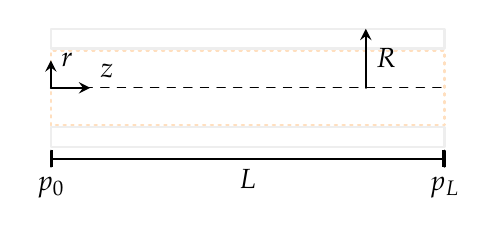
\begin{tikzpicture}[scale=0.5, line cap=round, line join=round, thick]

			% Layer thicknesses (adjust as needed)
			% Assume total thickness ~ 3 units, with top gray = 0.5, orange ~2, bottom gray=0.5
			\def\totalwidth{10} % horizontal length representing L
			\def\bottom{0}
			\def\middlelow{0.5}
			\def\middlehigh{2.5}
			\def\top{3.0}
		
			% Draw layers:
			% bottom grey layer
			\draw[w] (0,0) rectangle (10,0.5);
		
			% orange layer
			\draw[o1, dotted, thick] (0,0.55) rectangle (10,2.45);
		
			% top grey layer
			\draw[w] (0,2.5) rectangle (10,3.0);
		
			% Draw the black dashed line (datum line) near the middle of the orange layer
			\draw[dashed, thin] (0,1.5) -- (10,1.5);
		
			% Draw coordinate axes in the left portion:
			% z-axis horizontally along the dashed line
			\draw[-stealth, thick] (0,1.5) -- (1,1.5) node[above right] {$z$};
		
			% r-axis vertically upwards from left side
			\draw[-stealth, thick] (0,1.5) -- (0,2.2) node[anchor=west] {$r$};
		
			% Mark the radius R upwards from the dashed line
			\draw[-stealth, thick] (8,1.5) -- (8,3) node[midway,right] {$R$};
		
			% Draw boundary conditions for pressure at ends:
			% Left boundary line and label p_0
			\draw[thick] (0,-0.5) -- (0,-0.1); 
			\node[anchor=north] at (0,-0.5) {$p_0$};
		
			% Right boundary line and label p_L
			\draw[thick] (10,-0.5) -- (10,-0.1); 
			\node[anchor=north] at (10,-0.5) {$p_L$};
		
			% Draw dimension line for L
			\draw[|-|, thick] (0,-0.3) -- (10,-0.3) node[midway, below] {$L$};
		
		\end{tikzpicture}
	\end{center}
	Assuming $u_z = u_z(r)$, $u_r = u_\theta = 0$ and $p = p(z)$, the only non-vanishing component of the rate-of-deformation tensor is the $rz$-component. For generalized Newtonian flow, $\tau_{rz}$ is the only non-zero component of the viscous stress. The $z$-momentum equation then reduces to:

	\[
	\frac{1}{r} \frac{d}{dr} \left( r \tau_{rz} \right) = \frac{dp}{dz},
	\]

	where $\tau_{rz}$ is a function of $r$.

	From the symmetry argument, $\tau_{rz}(r)$ satisfies:

	\[
	\tau_{rz} = -m \left| \frac{du_z}{dr} \right|^{n-1} \frac{du_z}{dr},
	\]

	where $m$ and $n$ are material-specific parameters for the power-law fluid.

	The velocity profile is derived as:

	\[
	u_z(r) = \left( \frac{3n+1}{n+1} \right) \left[ 1 - \left(\frac{r}{R}\right)^{(n+1)/n} \right] \bar{u}_z,
	\]

	where $\bar{u}_z$ is the mean velocity defined as:

	\[
	\bar{u}_z = \frac{2}{R^2} \int_0^R u_z r \, dr.
	\]

	Finally, the volumetric flow rate is expressed as:

	\[
	Q = \pi R^2 \bar{u}_z = \left( \frac{n \pi}{3n+1} \right) \left[ \frac{R^{n+1}}{2m} \frac{dp}{dz} \right]^{1/n}.
	\]
\end{conceptbox}
\columnbreak
\begin{conceptbox}[w]{practice problems}
	$$\\
	\vspace{7.3in}
	$$\\
\end{conceptbox}
\end{multicols*}
\end{document}







